\documentclass[a4paper]{article}

\documentclass[a4paper]{article}
\usepackage[utf8]{inputenc}
\usepackage[spanish, es-tabla, es-noshorthands]{babel}
\usepackage[table,xcdraw]{xcolor}
\usepackage[a4paper, footnotesep = 1cm, width=20cm, top=2.5cm, height=25cm, textwidth=18cm, textheight=25cm]{geometry}
%\geometry{showframe}

\usepackage{tikz}
\usepackage{amsmath}
\usepackage{amsfonts}
\usepackage{amssymb}
\usepackage{float}
\usepackage{graphicx}
\usepackage{caption}
\usepackage{subcaption}
\usepackage{multicol}
\usepackage{multirow}
\setlength{\doublerulesep}{\arrayrulewidth}
\usepackage{booktabs}

\usepackage{hyperref}
\hypersetup{
    colorlinks=true,
    linkcolor=blue,
    filecolor=magenta,      
    urlcolor=blue,
    citecolor=blue,    
}

\newcommand{\quotes}[1]{``#1''}
\usepackage{array}
\newcolumntype{C}[1]{>{\centering\let\newline\\\arraybackslash\hspace{0pt}}m{#1}}
\usepackage[american]{circuitikz}
\usetikzlibrary{calc}
\usepackage{fancyhdr}
\usepackage{units} 

\graphicspath{{../Ejercicio-1/}{../Ejercicio-2/}{../Ejercicio-3/}{../Ejercicio-4/}}

\pagestyle{fancy}
\fancyhf{}
\lhead{22.01 Teoría de Circuitos}
\rhead{Mechoulam, Lambertucci, Rodriguez Turco, Londero, Galdeman}
\rfoot{\centering \thepage}

\usepackage{float}
\usepackage{graphicx}

\usepackage[american voltage]{circuitikz}

\usepackage{amsmath}

\usepackage{xcolor}

\usepackage{multirow}

\usepackage{caption}
\usepackage{subcaption}

\begin{document}

\subsection{Fisiología del oído}

La fisiología auditiva se encuentra dada en tres estructuras:
\begin{itemize}
	\item Oído externo:
	Este conforma parte del órgano periférico encargado de la conducción de estímulos externos, transmitiendolos hacia el canal auditivo externo. Las paredes rígidas de este último evitan que el sonido sea absorbido por por los demás tejidos blandos.
	\item Oído medio:
	Compuesto por el sistema timpanoosicular (membrana timpánica y los tres huesillos: martillo, yunque y estribo), cumple con la función tanto de transmitir las señales del ambiente, como de proteger las estructuras neurosensoriales del oído interno y de la ventana redonda.
	\item Oído interno:
	Constituido por el laberinto óseo y dentro de este, el membranoso. Comprende dos aparatos desde el punto de vista anatómico y funcional: el coclear, encargado de la audición y por ende, del desarrollo del lenguaje, y el vestibular, que es el órgano que se ocupa del equilibrio\footnote{Diamante, V. (2004). Otorrinolaringología y afecciones conexas. Buenos Aires: El Ateneo.}.
\end{itemize}

\begin{figure}[H]
\centering
	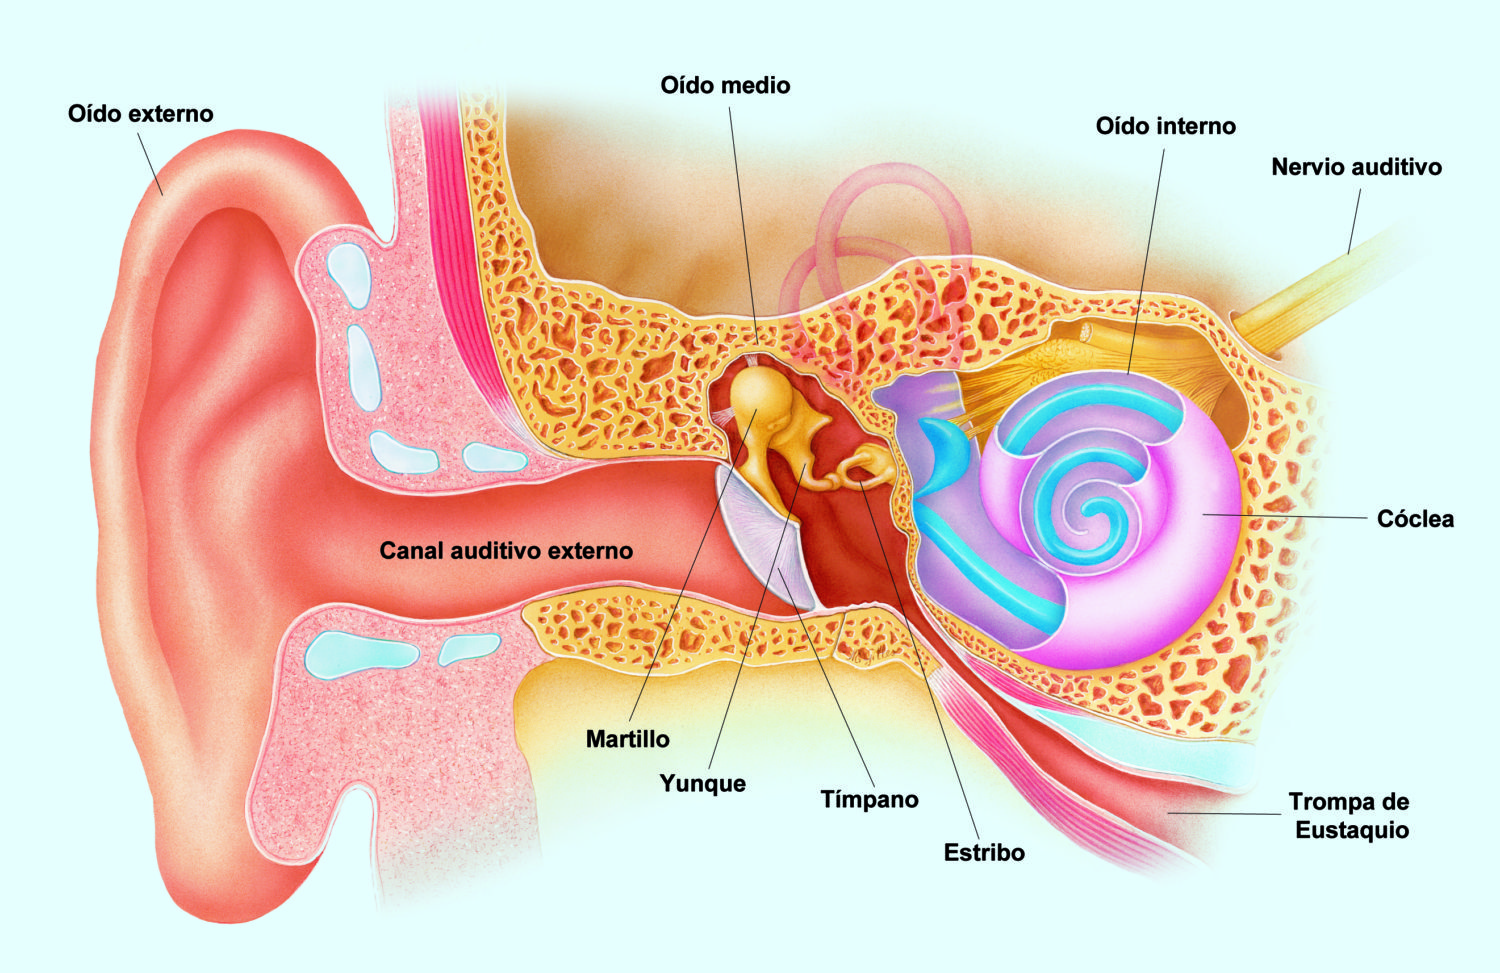
\includegraphics[width=0.9\textwidth]{Imagenes/Partes-del-oido.png}
	\caption{Estructura interna del oído.}
	\label{fig:oido}
\end{figure}

La señal captada se caracteriza por poseer una amplitud variable, la cual crece hasta alcanzar un máximo, para luego decrecer abruptamente. Además, dependiendo de la frecuencia de dicha onda, varía el sitio de la cóclea donde se presenta la máxima amplitud. De esta forma, el pico de amplitud se presenta en las inmediaciones del vértice de la cóclea para las frecuencias bajas (graves), mientras que para las altas (agudas), en la vecindad del vestíbulo.

El ser humano puede detectar frecuencias entre los $20 \ Hz$ y los $20 \ kHz$\footnote{En.wikipedia.org. (2019). Audio frequency. [online] Available at: https://en.wikipedia.org/wiki/Audio\_frequency [Accessed 11 Sep. 2019].}. A continuación, se realiza un detenimiento en el análisis de la ganancia del oído medio y externo. Es así que se muestra en la Figura (\ref{fig:oidoganancia}) la ganancia del oído externo, medio y la suma de ambas. Se destaca como las frecuencias menores a $1500 \ Hz$ no son prácticamente alteradas por el oído externo, mientras que la ganancia del oído medio se asemeja a un filtro pasa-banda al rededor de $1 \ kHz$. Finalmente, se puede decir que la suma de ambas converge en un gran filtro pasa-banda, cuyo pico máximo se encuentra cercano a los $3 \ kHz$. Es importante esta observación, ya que dicho filtro es el que determina el espectro audible por el ser humano\footnote{S. Rosen and P. Howell, Signals and systems for speech and hearing, 2nd ed. 2011.}. 

\begin{figure}[H]
\centering
	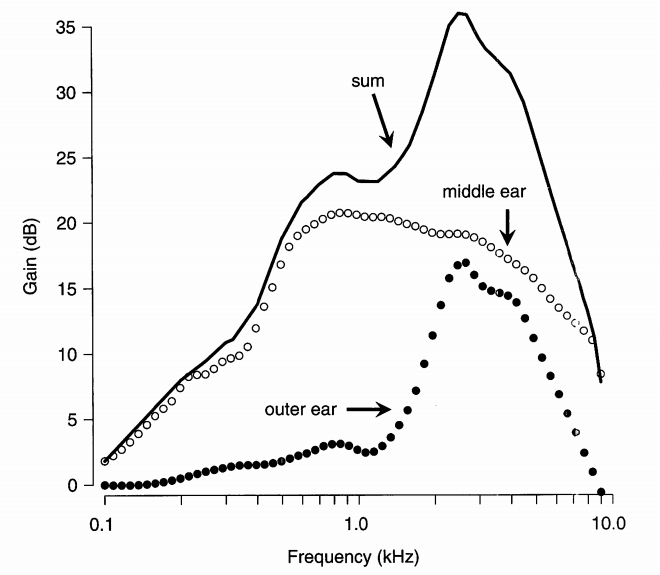
\includegraphics[width=0.9\textwidth]{Imagenes/Ganancia-del-oido-externo-y-medio.png}
	\caption{Ganancia del oído externo, medio y total.}
	\label{fig:oidoganancia}
\end{figure}

Es así que se presenta una división de las bandas de frecuencia audibles por el oído humano\footnote{``Ecualización Básica: Todo lo que necesitas saber sobre la Ecualización | LANDR Blog'', LANDR Blog, 2019. [Online]. Available: https://blog.landr.com/es/ecualizacion-basica-todo-lo-que-necesitas-saber-sobre-la-ecualizacion/. [Accessed: 11- Sep- 2019].}.

%\begin{table}[H]
%\begin{center}
%\hspace*{-2.75cm}
%\begin{tabular}{|c|c|c|c|c|c|}
%\hline
%\multicolumn{2}{|c|}{Bajos}           & \multicolumn{2}{c|}{Medios}           & \multicolumn{2}{c|}{Altos}                                                  \\ \hline
%Frecuencia [Hz]   & División          & Frecuencia [Hz]     & División        & Frecuencia [Hz]                        & División                           \\ \hline
%20 $\sim$ 40   & Graves profundos  & 300 $\sim$ 600   & Gama media-baja & \multirow{2}{*}{5000 $\sim$ 10000}  & \multirow{2}{*}{Gama alta}         \\ \cline{1-4}
%40 $\sim$ 80   & Graves bajos      & 600 $\sim$ 1200  & Gama media      &                                        &                                    \\ \hline
%80 $\sim$ 160  & Graves medios     & 1200 $\sim$ 2400 & Gama superior   & \multirow{2}{*}{10000 $\sim$ 20000} & \multirow{2}{*}{Gama extrema-alta} \\ \cline{1-4}
%160 $\sim$ 300 & Graves superiores & 2400 $\sim$ 5000 & Gama presencial &                                        &                                    \\ \hline
%\end{tabular}
%\caption{División del espectro de frecuencias audibles.}
%\label{table:divfreq}
%\end{center}
%\end{table}

\begin{figure}[H]
\centering
	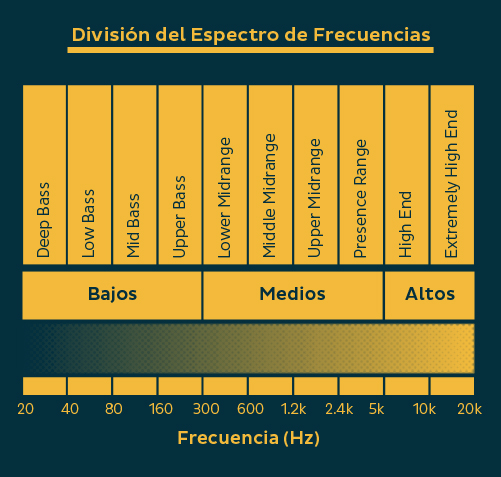
\includegraphics[width=0.7\textwidth]{Imagenes/FrequencySpectrumDivision.png}
	\caption{División del espectro de frecuencias audibles.}
	\label{fig:divfreq}
\end{figure}

Cabe destacar que las señales existentes en el ambiente pueden ser detectadas de dos formas distintas: mediante la vía aérea, es decir, a través el mecanismo explicado previamente, y mediante vibraciones óseas del cráneo. Mientras que el umbral de adución de la primera es teóricamente de $0 \ db$, la segunda posee un umbral mínimo de $60 \ db$. 

Para finalizar esta sección, se define cuando una persona sufre de una perdida de audición. Esta se da un individuo no puede oír o posee un umbral de audición mayor o igual a 25 dB. Para alcanzar esto, se debe superar el nivel máximo de exposición sin riesgos, el cual es de $85 \ dB$ durante 8 horas\footnote{"Escuchar sin riesgos!", Who.int, 2019. [Online]. Available: https://www.who.int/pbd/deafness/activities/MLS\_Brochure\_Spanish\_lowres\_for\_web.pdf. [Accessed: 11- Sep- 2019].}.

\subsection{Funcionamiento de un ecualizador}

Un equalizador es un dispositivo que se caracteriza por modificar la amplitud de los coeficientes de Fourier de una señal. En otras palabras, permite modificar la ganancia de de las frecuencias bajas, medias y/o altas de una señal. Para ello, se basa en la combinación de distintos filtros pasa-banda, cuya combinación permite dar con la configuración deseada.

Existen distintos tipos de ecualizadores, con mayor y menor cantidad de bandas, es decir, filtros selectores que amplifican o atenúan ciertas frecuencias. En el presente informe se desarrolló un filtro de tres bandas. Para ello se analizó el circuito brindado por la cátedra, mostrado en la Figura (\ref{fig:circuitoini}).

\begin{figure}[H]
\begin{center}
\begin{circuitikz}
	\node [op amp](A){};
	\draw (A.+) to[short] ++(-0.5,0) to[short] ++(0,-1) node[ground]{};
	\draw (A.-) to[short] ++(-0.5,0) to[short] ++(0,1.5) node[](v1){} to[R, l = $R_3$] ++(-3.5,0) to[short] ++(0,3);
	\draw (v1) to[R, l_= $R_3$] ++(3.5,0) to[short] ++(0,3);
	\draw (v1) to[open] ++(0,3) node[potentiometershape, rotate=180, label=south:$R_2$](P){};
	\draw (v1) to[C, l = $C_2$] (P.wiper);
	\draw (P.right) to[R, l= $R_1$] ++(-4,0) node[ocirc,label=left:$V_{in}$]{};
	\draw (P.left) to[R, l_= $R_1$] ++(4,0) node[ocirc,label=right:$V_{out}$]{};
	\draw (P.right) to[open] ++(-0.5,0) to[short] ++(0,1.5) to[C, l = $C_1$] ++(2.2,0) to[short] ++(0,-1.5);
	\draw (A.out) to[short] ++(0.62,0) to[short] ++(0,2);
\end{circuitikz}
	\caption{Circuito a analizar.}
	\label{fig:circuitoini}
\end{center}
\end{figure}

Para facilitar el análisis, se reemplaza el potenciometro $R_2$ con dos resistencias fijas, tal que se cumpla $R_2 = R_{2}^{'} + R_{2}^{''} $, considerando que
\begin{equation}
\begin{split}
	R_{2}^{'} &= \psi R_2\\ R_{2}^{''} &= \left( 1 - \psi \right) R_2
\end{split}
\label{equ:r2p}
\end{equation}
siendo $0 \leq \psi \leq 1$.

\begin{figure}[H]
\begin{center}
\begin{circuitikz}
	\node [op amp](A){};
	\draw (A.+) to[short] ++(-0.5,0) to[short] ++(0,-1) node[ground]{};
	\draw (A.-) to[short] ++(-0.5,0) to[short] ++(0,1.5) node[](v1){} to[R, l = $R_3$] ++(-3.5,0) to[short] ++(0,3);
	\draw (v1) to[R, l_= $R_3$] ++(3.5,0) to[short] ++(0,3);
	\draw (v1) to[C, l = $C_2$] ++(0,1.5) node[](v2){};
	\draw[color=red] (v2) to[short] ++(-1,0) to[R, l= $R_{2}^{'}$, color = red] ++(0,1.5) node[](v3){};
	\draw[color=red] (v2) to[short] ++(1,0) to[R, l_= $R_{2}^{''}$, color = red] ++(0,1.5) node[](v4){};
	\draw[color=red] (v3) to[C, l = $C_1$, color = red] (v4);
	\draw (v3) to[R, l= $R_1$] ++(-3,0) node[ocirc,label=left:$V_{in}$]{};
	\draw (v4) to[R, l_= $R_1$] ++(3,0) node[ocirc,label=right:$V_{out}$]{};
	\draw (A.out) to[short] ++(0.62,0) to[short] ++(0,2);
\end{circuitikz}
	\caption{Reemplazando $R_2$ por resistencias fijas.}
	\label{fig:kennelly1}
\end{center}
\end{figure}

Luego se aplica el teorema de Kennelly para transformar la conexión tipo Pi, marcada en rojo en la Figura (\ref{fig:kennelly1}), a una tipo T.
\begin{figure}[H]
\begin{center}
\begin{circuitikz}
	\node [op amp](A){};
	\draw (A.+) to[short] ++(-0.5,0) to[short] ++(0,-1) node[ground]{};
	\draw (A.-) to[short] ++(-0.5,0) to[short] ++(0,1.5) node[](v1){} to[R, l = $R_3$] ++(-3.5,0) to[short] ++(0,3);
	\draw (v1) to[R, l_= $R_3$] ++(3.5,0) to[short] ++(0,3);
	\draw[color=red] (v1) to[C, l = $C_2$] ++(0,1.5) to[generic, l = $Z_C$] ++(0,1.5) node[](v2){};
	\draw[color=red] (v2) to[generic, l_= $Z_A$] ++(-2,0) to[R, l= $R_1$] ++(-1.5,0) node[](aux2){};
	\draw (aux2) to[short] ++(-1,0) node[ocirc,label=left:$V_{in}$]{};
	\draw[color=red] (v2) to[generic, l = $Z_B$] ++(2,0) to[R, l_= $R_1$] ++(1.5,0) node[](aux1){};
	\draw (aux1) to[short] ++(1,0) node[ocirc,label=right:$V_{out}$]{};
	\draw (A.out) to[short] ++(0.62,0) to[short] ++(0,2);
\end{circuitikz}
	\caption{Resultado de aplicar el teorema de Kennelly por primera vez.}
	\label{fig:kennelly2}
\end{center}
\end{figure}

Siendo:
\begin{equation*}
	Z_{A} = \frac{R_{2}^{'}}{C_{1} R_{2} S + 1}
\end{equation*}	
\begin{equation*}
	Z_{B} = \frac{R_{2}^{''}}{C_{1} R_{2} S + 1}
\end{equation*}	
\begin{equation*}
	Z_{C} = \frac{C_{1} R_{2}^{''} R_{2}^{'} S}{C_{1} R_{2} S + 1}
\end{equation*}

Nuevamente se aplica Kennelly, pero esta vez para transformar una configuración del tipo T al tipo Pi. Se utiliza la conexión marcada en rojo en la Figura (\ref{fig:kennelly2}).
\begin{figure}[H]
\begin{center}
\begin{circuitikz}
	\node [op amp](A){};
	\draw (A.+) to[short] ++(-0.5,0) to[short] ++(0,-1) node[ground]{};
	\draw (A.-) to[short] ++(-0.5,0) to[short] ++(0,1.5) node[](v1){} to[short] ++(-1.5,0) node[](aux1){};
	\draw[color=red] (aux1) to[short] ++(-2,0) to[R, l = $R_3$] ++(0,3);
	\draw[color=red] (aux1) to[generic, l = $Z_{AC}$] ++(0,3) node[](v2){};

	\draw (v1) to[short] ++(1.5,0) node[](aux2){};
	\draw[color=red] (aux2) to[short] ++(2,0) to[R, l_= $R_3$] ++(0,3);
	\draw[color=red] (aux2) to[generic, l_= $Z_{BC}$] ++(0,3) node[](v3){};
	
	\draw (v2) to[generic, l = $Z_{AB}$] (v3);
	\draw[color=red] (v3) to[short] ++(2,0) node[](aux3){};
	\draw (aux3) to[short] ++(1,0) node[ocirc,label=right:$V_{out}$]{};
	
	\draw[color=red] (v2) to[short] ++(-2,0) node[](aux4){};
	\draw (aux4) to[short] ++(-1,0)node[ocirc,label=left:$V_{in}$]{};
	\draw (A.out) to[short] ++(0.62,0) to[short] ++(0,2);
\end{circuitikz}
	\caption{Resultado de aplicar el teorema de Kennelly por segunda vez.}
	%\label{}
\end{center}
\end{figure}

Obteniendose así:
\begin{equation*}
	Z_{AC} =  \frac{\alpha_{AC} {C_{1}}^{2} C_2 R_{1} R_{2} S^{3} + \beta_{AC} C_1 S^{2}
		+ \gamma_{AC} S + 2 R_1 + R_{2}^{'} + R_{2}^{''}}{
		 C_2 S \left( C_1 R_{2} S + 1 \right)
		\left(C_1 R_1 R_{2} S + R_1 + R_{2}^{''}\right)}
\end{equation*}
con
\begin{equation*}
\begin{split}
	\alpha_{AC} = R_{1} R_{2} + 2 {C_{1}}^{2} C_2 R_{2}^{'} R_{2}^{''}
\end{split}
\end{equation*}
\begin{equation*}
\begin{split}
	\beta_{AC} =\ & 2 C_{1} R_1 R_{2}^{2} + 2 C_2 R_{1}^{2} R_{2} + C_2 R_1 R_{2} R_{2}^{'} +
		C_2 R_1 R_{2} R_{2}^{''} + 2 C_2 R_1 R_{2}^{'} R_{2}^{''} + C_2 R_{2}^{'2} R_{2}^{''} + C_2 R_{2}^{'} R_{2}^{''2}\\
	\gamma_{AC} =\ & 4 C_1 R_1 R_{2} + C_1 R_{2} R_{2}^{'} + C_1 R_{2} R_{2}^{''} +
		C_2 {R_{1}}^{2} + C_2 R_1 R_{2}^{'} + C_2 R_1 R_{2}^{''} + C_2 R_{2}^{'} R_{2}^{''}
\end{split}
\end{equation*}

\begin{equation*}
	Z_{AB} = \frac{3 C_1 R_1 R_{2} S + 3 R_1 + 2 R_{2}^{'} + R_{2}^{''}}{C_1 R_{2} S + 1}
\end{equation*}

\begin{equation*}
	Z_{BC} =
	\frac{ \left( R_1 R_{2} + 2 R_{2}^{'} R_{2}^{''} \right ){C_{1}}^{2} C_2 R_1 R_{2} S^{3} +
	\beta_{BC} C_1 S^{2} + \gamma_{BC} S + 2 R_1 + R_{2}^{'} + R_{2}^{''}}
	{C_2 S \left(C_1 R_{2} S + 1\right) \left(C_1 R_1 R_{2} S + R_1 + R_{2}^{'} \right)}
\end{equation*}
con
\begin{equation*}
\begin{split}
	\beta_{BC} =\ & 2 C_1 R_1 {R_{2}}^{2} + 2C_2 {R_{1}}^{2} R_{2} + C_2 R_1 R_{2} R_{2}^{'} + C_2 R_1 R_{2} R_{2}^{''} + 2 C_2 R_1 R_{2}^{'} R_{2}^{''} + 
	C_2 {R_{2}^{'}}^2 R_{2}^{''} + C_2 R_{2}^{'} R_{2}^{''2}\\
	\gamma_{BC} =\ & 4 C_1 R_1 R_{2} + C_1 R_{2} R_{2}^{'} + C_1 R_{2} R_{2}^{''} +
	C_2 {R_{1}}^{2} + C_2 R_1 R_{2}^{'} + C_2 R_1 R_{2}^{''} +
	C_2 R_{2}^{'} R_{2}^{''} 
\end{split}
\end{equation*}

Luego, se toma el paralelo entre las impedancias marcadas en rojo en la Figura (\ref{fig:paralelo}).
\begin{figure}[H]
\begin{center}
\begin{circuitikz}
	\node [op amp](A){};
	\draw (A.-) to[short] ++(-1,0) to[generic, l = $Z_{AC}^{'}$, i<_ = $I_{C}$] ++(-2,0) node[](v1){} to[short, -o, i<_= $I_{in}$] node[ocirc,label=left:$V_{in}$]{} ++(-1,0);
	\draw[color=red] (v1) to[short] ++(0,2.5) to[generic, l = $Z_{AB}$, i = $I_{B}$] ++(6.5,0) to[short] ++(0,-3);
	\draw (A.+) to[short] ++(-0.5,0) to[short] ++(0,-1) node[ground]{};
	\draw (A.-) to[short] ++(-0.5,0) to[short] ++(0,1.5) to[generic, l_= $Z_{BC}^{'}$, i = $I_{C}$] ++(3,0) to[short] ++(0,-2);
	\draw (A.out) to[short, -o] ++(2,0) node[ocirc,label=right:$V_{out}$]{};
\end{circuitikz}
	\caption{Resultado de tomar las impedancias en paralelo.}
	\label{fig:paralelo}
\end{center}
\end{figure}

Es así que, definiendo: $Z_{AC}^{'} = Z_{AC} // R_3 $, $Z_{BC}^{'} = Z_{AC} // R_3 $, se plantean las siguientes ecuaciones:

\begin{equation*}
\left\{
\begin{aligned}
		& V_{out} = A_o \left( V^+ - V^- \right) =  -A_o V^- \\
		& V_{in} - Z_{AC}^{'} \ I_{C} = V^- \\
		& V^- - Z_{BC}^{'} \ I_{C} = V_{out}
\end{aligned}
\right.
\end{equation*}

Resolviendo el sistema previamente planteado, se llega a que la transferencia del circuito de la Figura (\ref{fig:paralelo}) corresponde a la de un amplificador inversor, por lo tanto, considerando (\ref{equ:r2p}), se obtiene:

\begin{equation*}
	H(S) = \frac{1}{\frac{Z_{BC}^{'}}{Z_{AC}^{'}} {A_{vol}\left(S\right)}^{-1} - \frac{Z_{BC}^{'}}{Z_{AC}^{'}} - {A_{vol}\left(S\right)}^{-1}} = \frac{1}{\frac{Z_{BC}^{'}}{Z_{AC}^{'}} \frac{1 + \frac{S}{\omega_o}}{A_{vol}} - \frac{Z_{BC}^{'}}{Z_{AC}^{'}} - \frac{1 + \frac{S}{\omega_o}}{A_{vol}}}
	\label{equ:hsavolw}
\end{equation*}

Tomando $\omega_o \rightarrow \infty$ se llega a

\begin{equation*}
	H(S) = \frac{1}{\frac{Z_{BC}^{'}}{Z_{AC}^{'}} {A_{vol}}^{-1} - \frac{Z_{BC}^{'}}{Z_{AC}^{'}} - {A_{vol}}^{-1}}
	\label{equ:hsavol}
\end{equation*}

Nuevamente, considerando $A_o \rightarrow \infty$ se obtiene

\begin{equation}
	H(s) = -\frac{Z_{BC}^{'}}{Z_{AC}^{'}} = - \frac{\alpha_H S^{2} + \beta_H S + 2 R_{1} + R_{2}}
	{\gamma_H S^{2} + \delta_H S + 2 R_{1} + R_{2}}
	\label{equ:hs}
\end{equation}

Siendo: 
\begin{equation*}
\begin{split}
	\alpha_H =\ & C_{1} C_{2} {R_{1}}^{2} R_{2} - 2 C_{1} C_{2} R_{1} {R_{2}}^{2} \psi^{2} + 2 C_{1} C_{2} R_{1} {R_{2}}^{2} \psi + C_{1} C_{2} R_{1} R_{2} R_{3}\\
	\beta_H =\ & 2 C_{1} R_{1} R_{2} + C_{2} {R_{1}}^{2} + C_{2} R_{1} R_{2} + C_{2} R_{1} R_{3} - C_{2} {R_{2}}^{2} \psi^{2} + C_{2} {R_{2}}^{2} \psi - C_{2} R_{2} R_{3} \psi + C_{2} R_{2} R_{3}\\
	\gamma_H =\ & C_{1} C_{2} {R_{1}}^{2} R_{2} - 2 C_{1} C_{2} R_{1} {R_{2}}^{2} \psi^{2} + 2 C_{1} C_{2} R_{1} {R_{2}}^{2} \psi + C_{1} C_{2} R_{1} R_{2} R_{3}\\
	\delta_H =\ & 2 C_{1} R_{1} R_{2} + C_{2} {R_{1}}^{2} + C_{2} R_{1} R_{2} + C_{2} R_{1} R_{3} - C_{2} {R_{2}}^{2} \psi^{2} + C_{2} {R_{2}}^{2} \psi + C_{2} R_{2} R_{3} \psi
\end{split}
\end{equation*}

Además, realizando el ensayo de circuito cerrado, se puede calcular la impedancia de entrada:
\begin{equation}
	Z_{in} = \frac{V_{out}}{V_{in}} = \frac{\left( Z_{AC}^{'} + Z_{BC}^{'} \right) \cdot Z_{AB}}{Z_{AC}^{'} + Z_{BC}^{'} + Z_{AB}}
	\label{equ:zin}
\end{equation}

Si se tienen en cuenta las siguientes consideraciones: $C_1 = 10 \ C_2$, $R_3 \gg R_1$ y $R_3 = 10 \ R_2$, se pueden reescribir los coeficientes de (\ref{equ:hs}), obteniéndose: 
\begin{equation*}
\begin{split}
	\alpha_H =\ \gamma_H =\ & 10 {C_{2}}^{2} {R_{2}}^{2} R_{1} \left[ 10 + 2 \psi \left(1 - \psi \right) \right]
\end{split}
\end{equation*}
\begin{equation*}
\begin{split}
	\beta_H =\ & C_{2} R_{2} \left[ 31 R_1 + R_2 \left(10 - 9 \psi - \psi^2 \right) \right]
\end{split}
\end{equation*}
\begin{equation*}
\begin{split}
 \delta_H =\ & C_{2} R_{2} \left[ 31 R_1 + R_2 \psi \left(11 - \psi \right) \right]
\end{split}
\end{equation*}

Es así que, con los nuevos coeficientes simplificados, se obtiene de (\ref{equ:hs}) la frecuencia de corte del filtro:
\begin{equation}
\begin{split}
	f_o &=\ \frac{1}{2 \pi} \sqrt{\frac{2R_1 + R_2}{\alpha_H}} = \sqrt{\frac{2R_1 + R_2}{10 {C_{2}}^{2} {R_{2}}^{2} R_{1} \left[ 10 + 2 \psi \left(1 - \psi \right) \right]}} = \\
	&=\ \sqrt{\frac{2 + \frac{R_2}{R_1}}{10 \left[ 10 + 2 \psi \left(1 - \psi \right) \right]}} \cdot \frac{1}{2 \pi C_2 R_2}
\end{split}
\label{equ:fogeneral}
\end{equation}

Tomando tanto $\psi = 1$, como $\psi = 0$ se obtiene la misma frecuencia de corte
\begin{equation*}
\begin{split}
	f_o &=\ \frac{\sqrt{2 + \frac{R_2}{R_1}}}{20 \pi C_2 R_2}
\end{split}
\end{equation*}

De esta forma, se busca la variación de amplitud máxima en dicha frecuencia. Esto se realiza evaluando la transferencia del sistema en $J\omega_o$, obteniendo de esta forma $A_{0Max}$ y $A_{0Min}$. Luego, tomando $\psi = 0$:
\begin{equation*}
\begin{split}
|H\left(J\omega_o\right)| = A_{0Max} = \frac{31 R_{1} + 10 R_{2}}{31 R_{1}} \approx \frac{30 R_{1} + 10 R_{2}}{30 R_{1}} = \frac{3 R_{1} + R_{2}}{3 R_{1}}
\end{split}
\end{equation*}

Por otro lado, con $\psi = 1$:
\begin{equation*}
\begin{split}
|H\left(J\omega_o\right)| = A_{0Min} = \frac{31 R_{1}}{31 R_{1} + 10 R_{2}} \approx \frac{30 R_{1}}{30 R_{1} + 10 R_{2}} = \frac{3 R_{1}}{3 R_{1} + R_{2}}
\end{split}
\end{equation*}

Se determina de esta forma que
\begin{equation*}
\begin{split}
\frac{3 R_{1}}{3 R_{1} + R_{2}} \leq A_0 \leq \frac{3 R_{1} + R_{2}}{3 R_{1}}
\end{split}
\end{equation*}

Además, mediante el uso de (\ref{equ:hs}), se calculan los respectivos polos y ceros del sistema, enfunción de $\psi$ y se realiza un diagrama de polos y ceros en el plano $S$, variando dicho factor. De esta forma se obtiene la Figura (\ref{fig:zplanepsi}).

\begin{figure}[H]
	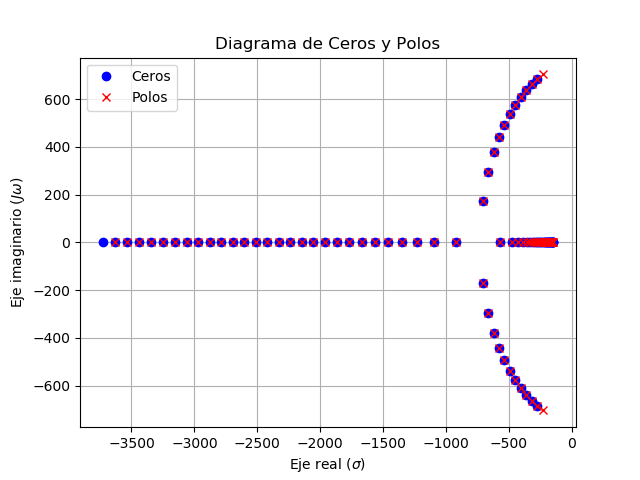
\includegraphics[width=\textwidth]{Imagenes/Zplanepsi.png}
\caption{Diagrama de polos y ceros variando $\psi$ entre 0 y 1.}
	\label{fig:zplanepsi}
\end{figure}

En un ecualizador analógico, al modificar una frecuencia dada, se modifica también su fase. Este es un proceso inevitable, el cual se busca reducir tanto como sea posible, buscando también lograr que produzca el cambio de tono deseado. Esto se garantiza realizando que el sistema sea de fase mínima.
Debido a que, tanto los polos como los ceros del sistema, sin importar el valor de $\psi$, se encuentran en el semiplano izquierdo, se obtiene el menor diagrama de fase posible, en consecuencia, este sistema es de fase mínima.

\begin{center}
\textcolor{red}{\textbf{BUSCAR HACERLO DE FASE NO MÍNIMA.}}
\end{center}

\subsection{Desarrollo del circuito y selección de componentes}

Teniendo en cuenta lo expresado en la primer sección, se procede a elegir frecuencias de corte para cada una de las instancias. Recordando el que el espectro auditivo del ser humano abarca desde los $20 \ Hz$ a los $20 \ kHz$, y considerando lo mostrado en la Figura (\ref{fig:divfreq}), se decide buscar una frecuencia representativa para cada parte del espectro (bajos, medios y altos). Debido al carácter logarítmico de las frecuencias, se calculan dichas frecuencias de la forma:
\begin{equation*}
	\log{(f_{med})} = \frac{\log(f_{min}) + \log(f_{max})}{2} = \log(\sqrt{f_{min} f_{max}})
\end{equation*}
Es así que se necesita una frecuencia cercana a los $77,50 \ Hz$ para las frecuencias bajas , $1,2 \ kHz$ para las medias y $10 \ kHz$ para las altas. De esta forma, y pensando en valores comerciales, se seleccionan los elementos deseados, completando la siguiente tabla:

\begin{table}[H]
\begin{center}
\begin{tabular}{ccccccc}
\hline
Banda & $R_1$ & $R_2$ & $R_3$ & $C_1$ & $C_2$ & $f_o$ \\
\hline
Baja & $1 \ k\Omega$ & $10 \ k\Omega$ & $100 \ k\Omega$ & $680 \ nF$ & $68 \ nF$ & $81,08 \ Hz$ \\
Media & $1 \ k\Omega$ & $10 \ k\Omega$ & $100 \ k\Omega$ & $47 \ nF$ & $4,7 \ nF$ & $1,17 \ kHz$ \\
Alta & $100 \ \Omega$ & $1 \ k\Omega$ & $10 \ k\Omega$ & $56 \ nF$ & $5,6 \ nF$ & $9,85 \ kHz$\\
\hline
\end{tabular}
\caption{Valores de los componentes seleccionados.}
\label{tabla:valores}
\end{center}
\end{table}

Una vez determinado esto, se optó por colocar las tres instancias en serie, ya que de esta forma se aprovecha mejor la amplificación de cada una, debido al hecho de que cada etapa solo amplifica o atenúa en un rango de frecuencias dadas, mientras que fuera de dicho rango, no se ven afectadas. Además, se buscó reproducir los valores de amplificación de ecualizadores comerciales, los cuales se encuentran entre $\pm 12 \ db$ y $\pm 15 \ db$.
En consecuencia, la transferencia total del circuito resulta del producto de la de cada etapa, obtenida de reemplazar los valores mostrados en la Tabla (\ref{tabla:valores}) en (\ref{equ:hs}), mientras que la impedancia de entrada total del sistema resulta de la suma de cada impedancia de entrada, obteniendo esta de la misma forma que la tranferencia, es decir, tomando nuevamente los valores de la tabla previamente mencionada y reemplazandola en (\ref{equ:zin}). Es así que se procede a graficar la respuesta en frecuencia de todo el circuito, variando el factor $\psi$ para una instancia por vez, fijando los demás en $0,5$.
\begin{figure}[H]
\centering
	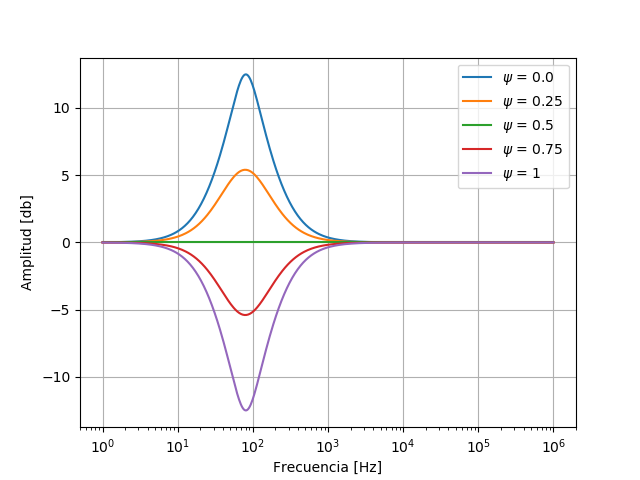
\includegraphics[width=0.9\textwidth]{Imagenes/Low-psi-bode.png}
	\caption{Diagrama de BODE en amplitud, variando $\psi$ de las frecuencias bajas.}
	\label{fig:bode_modulo_low}
\end{figure}
\begin{figure}[H]
\centering
	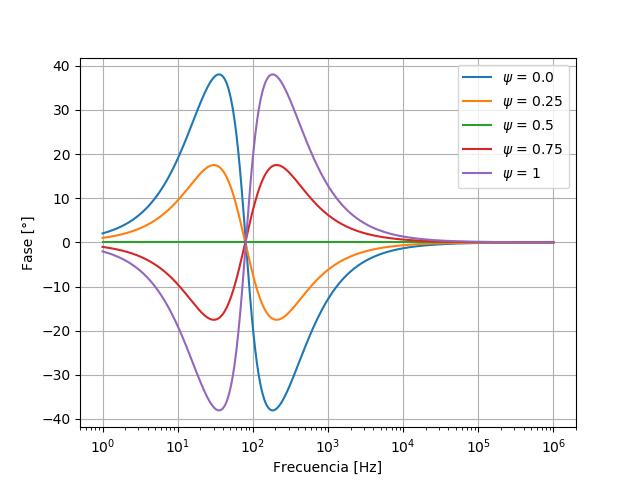
\includegraphics[width=0.9\textwidth]{Imagenes/Low-psi-ph.png}
	\caption{Diagrama de BODE en fase, variando $\psi$ de las frecuencias bajas.}
	\label{fig:bode_ph_low}
\end{figure}
\begin{figure}[H]
\centering
	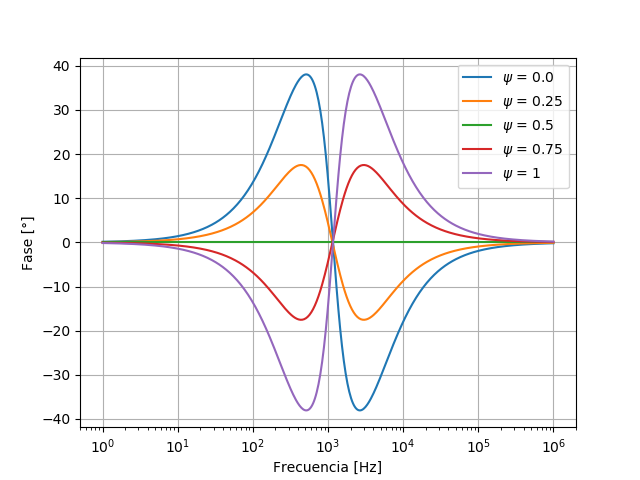
\includegraphics[width=0.9\textwidth]{Imagenes/Medium-psi-bode.png}
	\caption{Diagrama de BODE en amplitud, variando $\psi$ de las frecuencias medias.}
	\label{fig:bode_modulo_med}
\end{figure}
\begin{figure}[H]
\centering
	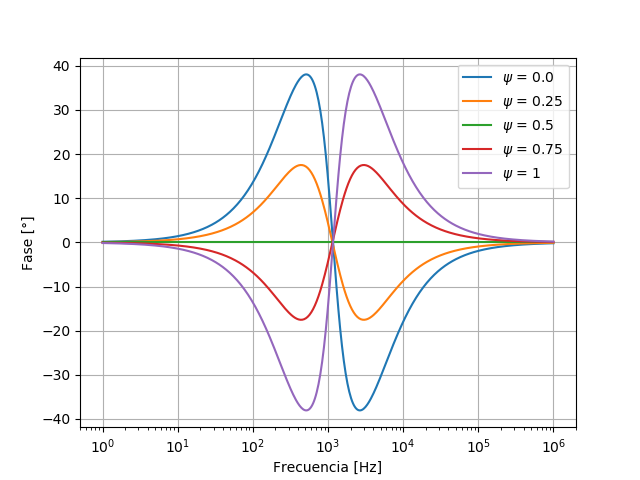
\includegraphics[width=0.9\textwidth]{Imagenes/Medium-psi-ph.png}
	\caption{Diagrama de BODE en fase, variando $\psi$ de las frecuencias medias.}
	\label{fig:bode_ph_med}
\end{figure}
\begin{figure}[H]
\centering
	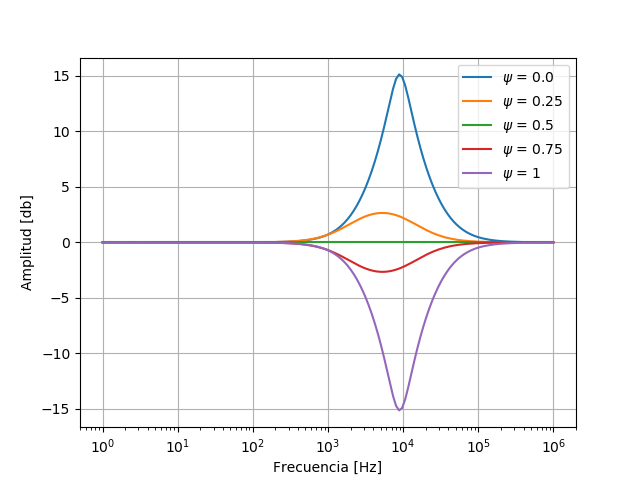
\includegraphics[width=0.9\textwidth]{Imagenes/High-psi-bode.png}
	\caption{Diagrama de BODE en amplitud, variando $\psi$ de las frecuencias altas.}
	\label{fig:bode_modulo_high}
\end{figure}
\begin{figure}[H]
\centering
	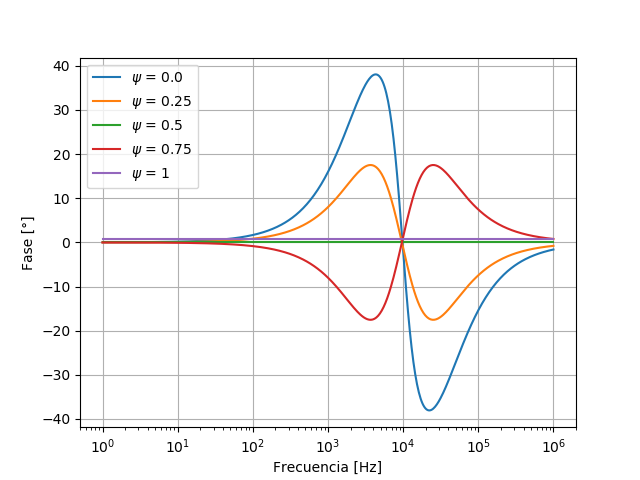
\includegraphics[width=0.9\textwidth]{Imagenes/High-psi-ph.png}
	\caption{Diagrama de BODE en fase, variando $\psi$ de las frecuencias altas.}
	\label{fig:bode_ph_high}
\end{figure}

\begin{center}
\textcolor{red}{\textbf{PONER ALGUNA CONCLUSIÓN U OBSERVACIÓN.}}
\end{center}

De la misma forma, se muestra la impedancia de entrada en función de la frecuencia para el circuito total. Debido a que se colocaron las tres instancias en serie, $Z_{In_{T}}$ es la suma de impedancia de cada instancia.
\begin{figure}[H]
\centering
	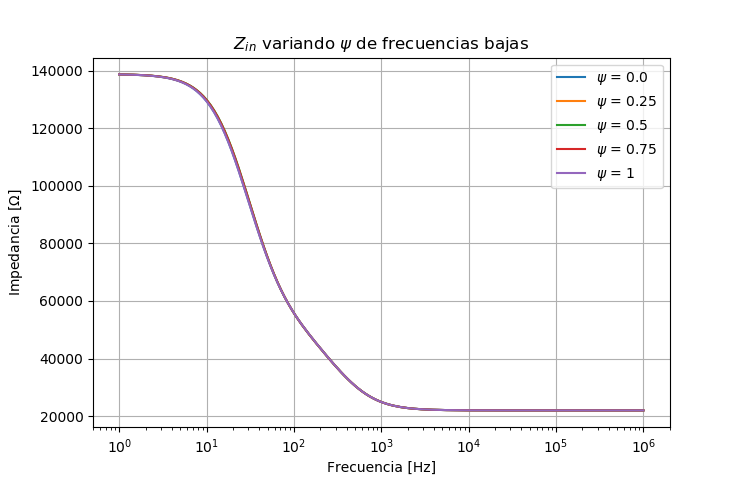
\includegraphics[width=0.9\textwidth]{Imagenes/Zin-Low-Mod.png}
	\caption{Impedancia de entrada en modulo, variando $\psi$ de las frecuencias bajas.}
	\label{fig:zin_modulo_low}
\end{figure}
\begin{figure}[H]
\centering
	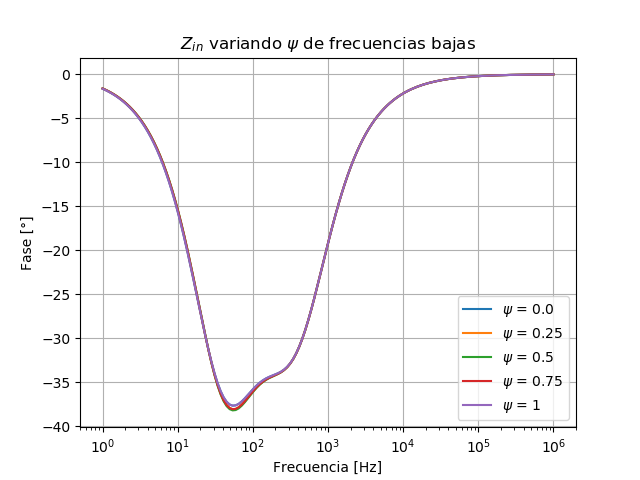
\includegraphics[width=0.9\textwidth]{Imagenes/Zin-Low-Ph.png}
	\caption{Fase de la impedancia de entrada, variando $\psi$ de las frecuencias bajas.}
	\label{fig:zin_ph_low}
\end{figure}
\begin{figure}[H]
\centering
	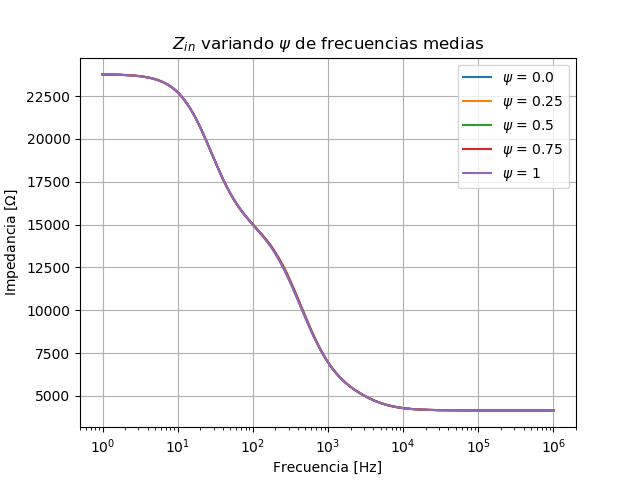
\includegraphics[width=0.9\textwidth]{Imagenes/Zin-Med-Mod.png}
	\caption{Impedancia de entrada en modulo, variando $\psi$ de las frecuencias medias.}
	\label{fig:zin_modulo_med}
\end{figure}
\begin{figure}[H]
\centering
	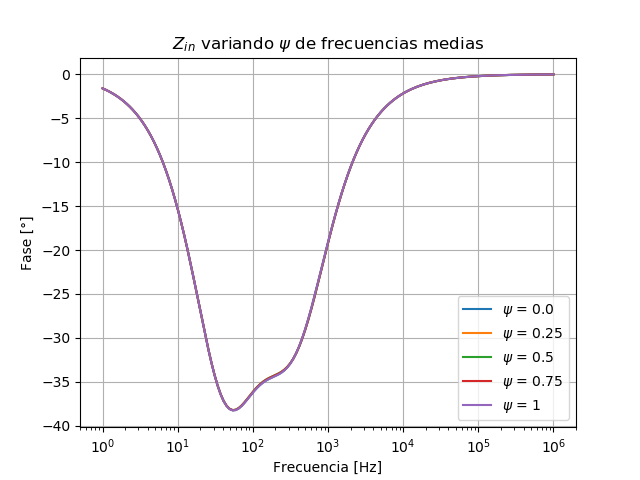
\includegraphics[width=0.9\textwidth]{Imagenes/Zin-Med-Ph.png}
	\caption{Fase de la impedancia de entrada, variando $\psi$ de las frecuencias medias.}
	\label{fig:zin_ph_med}
\end{figure}
\begin{figure}[H]
\centering
	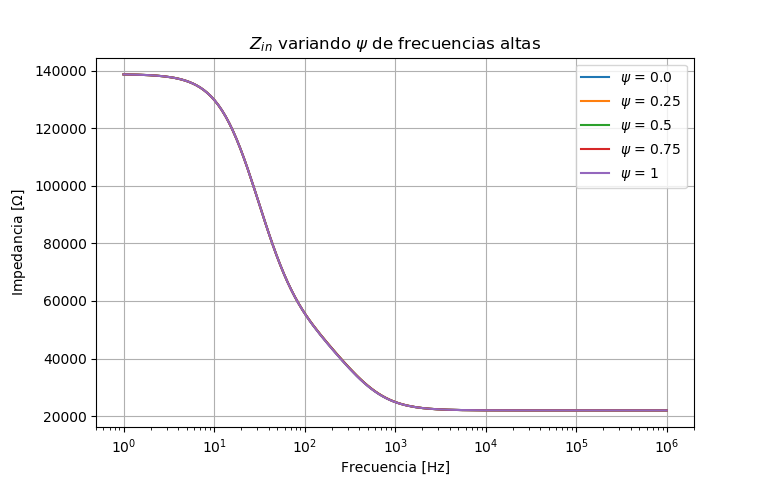
\includegraphics[width=0.9\textwidth]{Imagenes/Zin-High-Mod.png}
	\caption{Impedancia de entrada en modulo, variando $\psi$ de las frecuencias altas.}
	\label{fig:zin_modulo_high}
\end{figure}
\begin{figure}[H]
\centering
	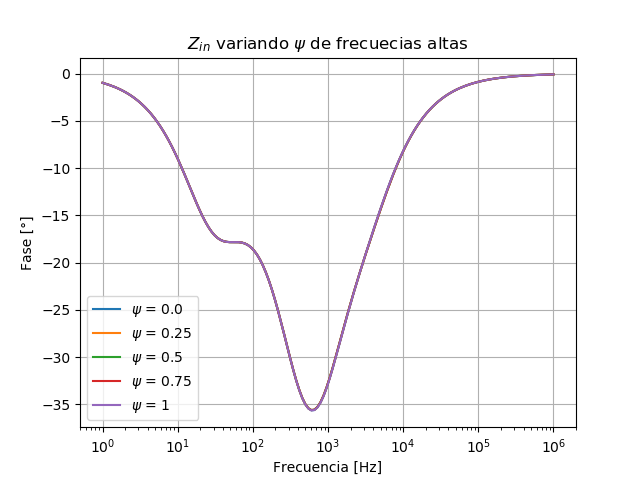
\includegraphics[width=0.9\textwidth]{Imagenes/Zin-High-Ph.png}
	\caption{Fase de la impedancia de entrada, variando $\psi$ de las frecuencias altas.}
	\label{fig:zin_ph_high}
\end{figure}


\end{document}